\documentclass{article}
\usepackage{graphicx}
\usepackage{amsfonts}
\usepackage{url}
\usepackage{pdfpages}
\usepackage{amsmath,amssymb}
\usepackage{enumerate}
\usepackage{color}
\usepackage{amsthm,amsmath}
\usepackage{bbm}
\usepackage{mhchem}

%for stacking below a sum or max...
\usepackage{mathtools}

\usepackage[colorlinks]{hyperref}

\newcommand{\comment}[2]{\vspace{0.6cm}{\bf Comment:} {\it #1.}

\vspace{0.3cm}{\bf Answer:} #2}

\begin{document}
\title{Response to Referee Comments: Parallel Adaptive Importance Sampling}
\maketitle
First of all, we would like to thank the referees and the associate editor for
their time in reading and commenting on our manuscript. In this document
we will address each of the points raised, and describe any relevant
changes that have been made to the paper. We have made some substantial changes, not least with the inclusion of a new ``large scale'' example where the likelihood requires a solve of a differential equation. We demonstrate in this example that PAIS is 2 orders of magnitude faster, in terms of CPU time, than the equivalent standard MCMC. We include a copy of the manuscript with all of the changes marked.

\section*{Referee 1 comments}

\comment{The PAIS algorithm does exhibits interesting ideas to combine the information 
obtained from an ensemble of proposals. Furthermore, it seems quite flexible 
since several proposals and re-sampling methods can be used.

However, the examples somehow fail to convince that the algorithm can be used 
in a wide range of challenging inverse problems. The approach is limited by the 
dimensionality of the problem.}{We thank the referee for their comments. We are very open about the fact that this approach cannot be used for high dimensional problems, but there are a plethora of lower dimensional inverse problems which exhibit structure in the posterior, such as multimodality or high correlations, for which existing MCMC methods struggle to converge in reasonable time. Dimensionality is not the only challenge faced in inverse problems, and these methods have been developed to tackle problems of a different nature. In particular, this method was designed with a view to sampling from inverse problems arising in Biology, where challenging posteriors exist on relatively low dimensional state spaces, and for which the likelihood can be very expensive to compute. We have added some words on this to clarify further the intended type of problem that this method is in the introduction, and again in the discussion at the end.}  %done

\comment{For mixture problems, if the mixture has to many 
elements (or the number of elements is unknown), then this scheme will have 
difficulties.}{This is true, as would state-of-the-art Riemannian manifold MALA, HMC and a whole range of other methods. I would be happy for the referee to indicate a method which would comfortably deal with a mixture problem with a large number of possible known/unknown components. The example was chosen to demonstrate the remarkable performance of the algorithm (with respect to standard MCMC methods) for multimodal posteriors in low dimensions, and we believe it has achieved that. We have added a paragraph to the end of the example to discuss the point that the referee makes.}%done

\comment{Also, it is not clear how it will behave in real life inverse 
problems where the likelihood is determined by complex physical systems that 
involve, for example, ODE's or PDE's. If the likelihood is expensive to 
evaluate, the tunning of the scaling parameters for the PAIS-RW might be a 
concern when the number of chains is big.}{The tuning of the scaling parameters is actually very fast, often converging within a few percentage points of the optimum within the order of $10^2$ iterations. We have included some plots and discussion to the end of Section 4.2 to demonstrate this point, and we thank the referee for highlighting this issue. This is quicker than one might expect for an adaptive serial algorithm.}%done

\comment{An real data example for the PAIS algorithm is much needed. It will be 
interesting to see how PAIS is compared not only against a naive 
parallelization, but also compared against a state of the art MCMC algorithm 
or/and a efficient ad hoc MCMC algorithm designed for such example.}{Unfortunately we do not have the resources to apply our method to a full-scale real data example. However, following additional comments from the editor, we have included a new example where the likelihood requires the solution of an ODE. In Section 7.5 we include an example of data assimilation for the Lorenz '63 equations, which is a set of equations which is commonly used to test methods for inference in the applied mathematics community. 

Expensive likelihoods actually make this method more applicable, since they make the extra overheads of the resampling step relatively less important. This is precisely what the method is designed for, and is the very reason for us to compare the algorithms by looking at error as a function of the number of samples/likelihood evaluations. This is seen even for a simple 3D ODE as we see in our example in Section 7.5, where PAIS reaches a relative error in the mean of $10^{-5}$ in a time which is 2 orders of magnitude quicker in CPU time than for trivially parallelised RWMH chains.}%done

\comment{There aren't details about the architecture used to run the M chains in 
parallel. This is relevant since there are several options such as: multi-core 
and multi-processor computers, GPU cards, clusters, cloud computing, etc. 
Comments about the advantages and disadvantages of the architecture 
are also welcome. The same goes for details regarding the programming language 
used.}{We thank the referee for this comment, as we should have included these details in the manuscript. The method was implemented in C++, serially, and was run on a single core of a Dell server with four 8-core 3.3GHz CPUs, 64Gb memory, and these details have been added in Section 7. 

We are not computer scientists, and as such, we are not in a position to comment on specific architectures, especially as the optimal architecture would be problem specific. The optimal architecture would likely depend on the relative costs of communication of the states across the processors, the cost of the likelihood evaluation, and the cost of the resampler for the chosen ensemble size. We have added a discussion to Section 3, following the presentation of the PAIS algorithm.}%done

\comment{CPU time must be reported to compare the gain of each algorithm in 
order to have a fair comparison. Authors claim that there is a significant 
gain in terms of the number of iterations needed to achieve a desire 
tolerance; examples in sections 7.2 and 7.3 show that PAIS saves up to 90\% of 
the iterations. However, if the CPU time needed to run 10 PAIS iterations is 
ten times the time needed to run 100 RWMH iterations, then the gain is not as 
good as presented. PAIS iterations are more time consuming than RWMH iterations 
due to the re-sampling step. The authors mentioned that the re-sampling step is 
computationally expensive and that is why they proposed the AMR re-sampling 
method. CPU time is of particular importance in example 7.4 since the number of 
parallel chains grows from 50 to 500.}{The referee may have missed Figure 5.1 in which we show the computational cost, in time, of the resamplers that we use in the paper, both the optimal transport resampler, and the AMR. As mentioned before in response to another of the referee's comments, we had neglected to share the specs of the machine that these times were recorded on, and this has now been added. % There is an additional cost in the algorithm over and above the resampler, which is the computation of the denominator in the weights, as pointed out by the second referee. If we have $M$ members of our ensemble, then the cost of this denominator across the whole ensemble is $M^2$, but it can be easily parallelised. We include some timings of the cost of this aspect of the algorithm in Section ****, and a discussion of the overall additional cost of the approach. 
% Coupled with the timings presented for the resampler, we believe that this now gives the reader a clear idea of the additional overhead costs which are incurred when using our method as opposed to a standard MCMC method. We thank the referee for their comments on this.

The reason for analysing the error as a function of the number of the likelihood evaluations, is that this method is intended for problems with expensive likelihoods, for which these overhead costs would be dwarfed. We have added a discussion on this to the beginning of Section 7.

Additionally to this, in Section 7.5, as detailed above, we have compared the CPU time that it takes the PAIS to reach a relative error in the mean of the posterior of $10^{-5}$ against that for trivially parallelised (non-communicative) RWMH. Even for a simple example such as this, PAIS outperforms standard parallelised MCMC by two orders of magnitude.}%done



\section*{Referee 2 comments}

\comment{This work in an interesting contribution in the field of Monte Carlo algorithms. The paper is technically sound and well-written. 
Moreover, it is possible to note the effort nd the care devoted by the authors.}{We thank the referee for their kind comments.}

\comment{However, I have some concerns. 

1) The starting-point algorithm in Table 1, is very similar to the basic scheme suggested in, for instance, 

V. Elvira, L. Martino, D. Luengo, M. F. Bugallo, Improving Population Monte Carlo: Alternative Weighting and Resampling Schemes, Signal Processing Vol. 131, pp. 77-91, 2017. 

In practice, you use a deterministic approach for the IS weights. 
I believe that the authors have analyzed and studied this idea independently, but this similarity should be discussed in the introduction, at least. 
You can also point out that you also propose some different resampling or adaptation schemes that are not contained in the previous work.}{We agree that there are similarities to this other work, and we thank the referee for their comment. Additional references have been added, along with more detailed discussions about the novel aspects of this manuscript in the introduction and discussion.}

\comment{2) I do not understand why you use the word "parallel" in the name of the algorithm. In Algorithm 1, it is difficult to recognize the parallelization. The denominator in the weight that you employ, in fact, is a bottleneck for a possible parallelization. Please clarify this point (even in the text).}{We have added clarifications on this point to Section 3. The referee should note that in our convergence plots, the reason that we compare the algorithms with respect to the number of likelihood evaluations is that we envisaged that this method would be of most use when the likelihood is expensive, for example when it requires a high resolution approximation of the solution of a PDE, and/or there is a very large amount of data to be taken into account. In this context, it would be useful to spread the work of computing the likelihood for the ensemble members across a cluster, hence our use of the word ``parallel''. We acknowledge and thank the referee for indicating the issues with the denominator. In the case where the likelihood is expensive, these overhead costs, along with that of the resampler, should no longer be the bottleneck. This was not adequately explained in the text, and as such we have added a further discussion in Section 3.

% We agree with this comment from the referee, as it may not have been made clear enough. With an ensemble of states, it is possible to distribute the computation of the weights across a set of cores. We have added a comment on this to Section ****. However, as discussed in the response to the first referee, we ourselves implemented the algorithm serially. Therefore, we have decided to change the name of the algorithm to reflect this, to ``Optimal Transport Adaptive Importance Sampling'' or OTAIS. Changes throughout the manuscript have been made to reflect this.
}

\comment{3) Please, add a table of acronyms that can help the reader. Now it is a bit confusing.}{We have added a glossary of acronyms to an appendix.} %half done -  complete

\comment{4) The references should be completed with other important contributions (considering also the same kind of weights, in some cases): 

- O.Cappe, R.Douc, A.Guillin, J.M.Marin, C.P.Robert, Adaptive importance sampling in general mixture classes, Statistics and Computing 18 (2008) 447-459. 
- R. Douc, A. Guillin, J. M. Marin, C. P. Robert, Convergence of adaptive mixtures of importance sampling schemes, Annals of Statistics 35 (2007) 420-448. 
- R. Douc, A. Guillin, J. M. Marin, C. P. Robert, Minimum variance importance sampling via population Monte Carlo, ESAIM: Probability and Statistics 11 (2007) 427-447. 
- L. Martino, V. Elvira, D. Luengo, J. Corander, Layered Adaptive Importance Sampling, Statistics and Computing, Vol. 27 (3), pp. 599-623, 2017.}{We thank the referee for thier suggestions for other highly relevant references.} %done

\section*{Associate Editor comments}
\comment{A very similar version of the authors’ PAIS algorithm has been studied before, as explained by the second referee. Moreover, I could argue that the PAIS algorithm is a particular case since weights are considered deter- ministic. This is a serious issue in the paper, let alone that the authors are unaware of the series of papers mentioned by referee 2, that are closely related to their work.
This should be explained in detail and the paper original perspective and contributions be further highlighted.}{Following suggestions by the second referee and the associate editor, we have added a significant new section to the introduction to highlight the other ensemble importance schemes already in the literature. We have also highlighted further the contribution made by this manuscript in the introduction and discussion sections.}%done

\comment{An other serious concern is why not use PMC-MCMC for the updating scheme in Algorithm 1. That would be as costly (since it also involves evaluating the posterior) but the yis will have the correct distribution.}{This comment is not clear to us - what is the ``updating scheme'' in Algorithm 1? Also, the (weighted) $y_i$ are distributed according to the posterior, as discussed in Section 6. We'd be happy to address this point if the AE is able to clarify it for us.}%nothing to do

\comment{The ”automatic” tuning will be as useful as the what traditional adaptive tuning is: in the limit, the proposal cov matrix converges to the cov matrix of the target. This is ok for Gaussian type targets but will fail for multimodal, multiscale distributions, mostly present in non-trivial forward maps, as those suggested in section 2. Something similar happens with gradient based proposals, since from the onset they are not conceived to scape local maxima.}{This is an interesting point, and the subject of our most recent paper in this area, in which transport maps are used to stabilise and accelerate the PAIS methodology, and also addressing exactly the point raised by the AE. We have added a discussion on this topic in the discussion section, proposing it as an area for future study (our new manuscript will be completed in the next few weeks).}%done

\comment{In Algorithm 1, note that in step 5 the actual number of different particles could be drastically reduced and in some cases collapsed to 1. As mentioned by the authors, this is a basic concern in SIR type algorithms, that they may become totally inefficient. Then, why this seems not to bother the authors and no provision was included in their algorithm to mend this problem?}{Provision is made within the code for such a catastrophic collapse of the weights, and it was remiss of us not to include details on this. We have added details on this to the end of Section 3.}%done

\comment{The Radon-Nokodyn version of Bayes theorem in (2.3) is unnecessary in the actual finite dimensional context the authors work with. The authors should state that, although there is an infinite dimensional version for the posterior distribution, their discussion is restricted to the parametric, finite dimensional case.}{We thank the AE for this comment. There is no need for this version of Bayes' theorem here, and so we have switched to the finite dimensional version.}%done

\comment{Note that in (2.4) the total measure of the space for ηˆ is M (!).}{Thanks to the AE for picking up on this typo, this has now been fixed.}%done


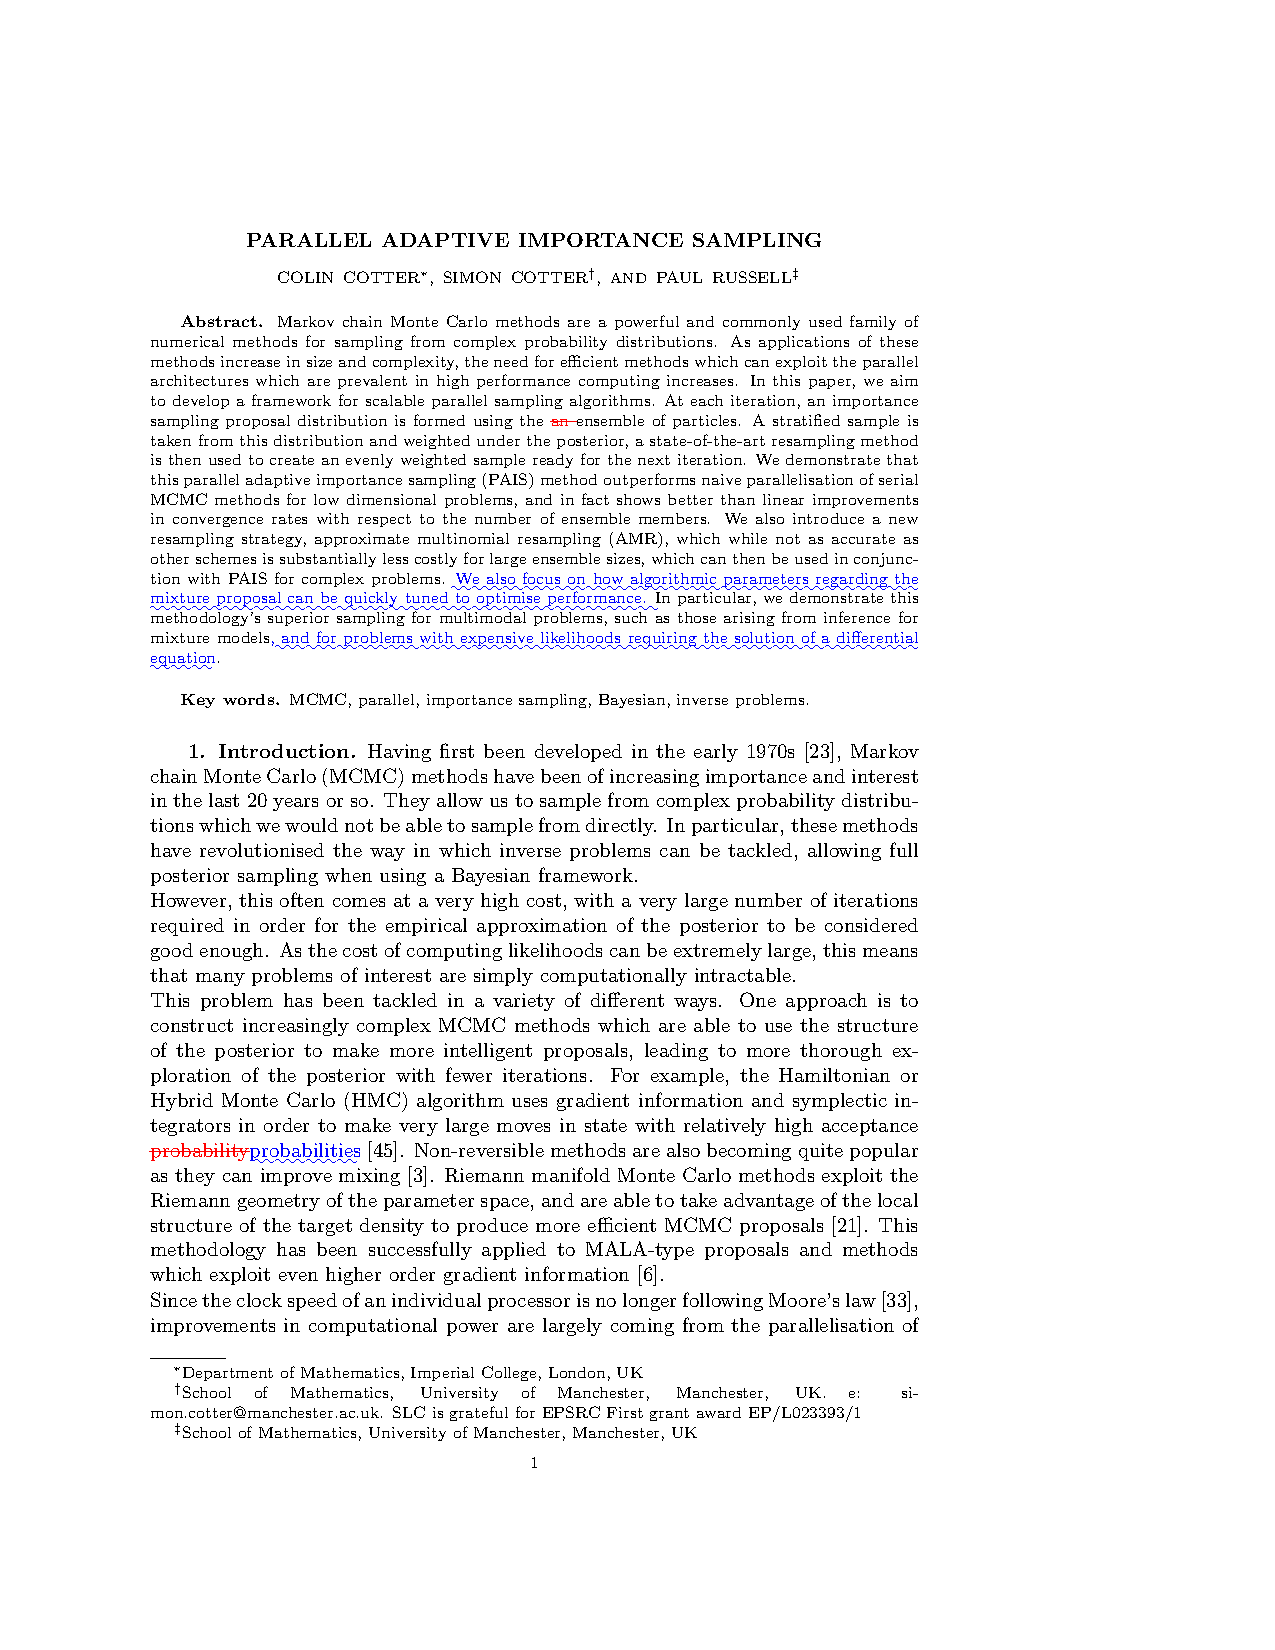
\includepdf[pages=-]{diff.pdf}

\end{document}
